A key part of this thesis is to advance the area of visualisation of medical imaging.
Even though techniques exist, operations are still planned on two-dimensional images for three-dimensional surgical sites.
\newline
As VR technology advances and entry costs are reduced, VR is considered more and more for a wide spectrum of applications.
In surgery, the main focus of research is on surgical training with pre-modeled patient anatomy and pathology.
By using state-of-the-art medical imaging and virtual reality technology and head mounted displays, this thesis aims to advance medical visualisation and surgery planning for patient specific procedures.
In Section \ref{sec::General}, a number of VR-based surgical simulations in different medical fields will be presented.
In Section \ref{sec::OralAndMaxillofacial}, the OMFS specific training tool "VR Surgery" will be presented.
VR Surgery was developed as a visualisation aid for senior surgeons and as a practice tool for novices.

\subsection{\label{sec::Devices}Used Devices}
\textbf{Devices}: Even though a wide range of devices are summarized as VR HMDs, there are just a few immersive HMDs, which allow the visualization of 3d models and interaction with their environment and the user thorugh technologies such as hand tracking or controllers.
\newline
Two particularly widespread devices are Oculus Rift \cite{OculusRift} and HTC Vive \cite{Vive}.
They are the first consumer HMDs widely known for their interaction and immersion compatibilities, bringing immersive VR to the consumer market around 2016.
For surgical purposes, HMDs like the Oculus Rift, including the developement kits DK 1 and 2 \cite{Parham.2019, Pulijala.2017,Sampogna.2017}, HTC Vive \cite{.2017, Barber.2020}, but also more recent devices such as Oculus Rift S (Quellen) were used.
\newline
One reason Oculus Rift head-mounted display was selected was its availability, cost and efficiency at the time of research \cite{Pulijala.2017}.
\newline
In the sense of augmented virtuality \cite{milgram1994taxonomy}, there exist different technologies for representation of the users hands in VR.
One such technologie is Leap Motion, which captures the users hands through the use of two cameras \cite{LeapMotion}.
These were applied in the surgical field to immerse users in the simulation \cite{Pulijala.2017, Sampogna.2017}
\newline
However, the use of consumer HMDs together with more specialized, non consumer haptic feedback devices such as the Geomagic Touch were also described in studies \cite{VenkataS.Arikatla.2018}.
Here, haptic feedback devices are used to improve the realism of surgical simulations. 
Advantages of such devices are a more realistic representation of the surgical procedure, while effectively having a higher barrier of entry.

\subsection{\label{sec::Input}Input Devices and Haptic Feedback}
[Hand tracking? Controller?]

\subsection{\label{sec::Visualization}Visualization of Anatomy}
Advancements in computers and imaging, especially over the last 10 years, have permitted the adoption of 3-dimensional imaging protocols in the health care field.
\newline
Virtual patients can be created by patient-specific anatomic reconstruction (PSAR), which can then be studied and used to develop and simulate treatment protocols.
Schendel et. al. propose image fusion, which involves combining images from different imaging modalities tocreate a virtual record of an individual called a patient-specific anatomic reconstruction \cite{schendel2009three}.
By using the combination of different image acquisition techniques, a treatment was planned for a young woman with mandibular retrusion.
It was shown that using generated 3D models of the patients specific anatomy and pathalogy brought huge improvements in planning treatments over traditional methods \cite{schendel2009three}.

In another related work, Computet Tomography (CT) and Magnetic Resonance (MR) were compared on the diagnostic potential in the aassessment of Synovia Chondromatosis (SR) of the Temporo-Mandibular Joint (TMJ).
Testaverde et al compared softtissueinvolvement (disk included), osteostructural alterations of the joints, loose bodies and intra-articular fluid of eight patients with symptoms of SC \cite{testaverde2011ct}.         
Results showed that CT scan is excellent to define bony surfaces of the articular joints and flogistic tissue but it fails in the detection of loose bodies when these are not yet calcified.
Optimally, a PSAR approach as proposed by Schendel et al \cite{schendel2009three} should be used.

\subsection{\label{sec::Video}Use of Video in Virtual Reality}
[Gefilmt, 3D]

\subsection{\label{sec::Interactions}Interactions}
[Instrumente usw.]

\subsection{\label{sec::Immersion}Immersion}
[Echter OP Raum]

\subsection{\label{sec::MultiUser}Multi User}
\textbf{Multi User Capability}:

\subsection{\label{sec::TissueSimulation}Tissue Simulation}
\input{sections/2_related_work/subsections/tissue_simmulation.tex}

\subsection{\label{sec::SurgicalSimulations}Developed Software}
At this point, the aforementioned six procedures are implemented in the system.
However, as described in Section \ref{sec::Architecture}, the system is extensible in the regard that new instruments can be implemented.
Currently, the implemented instruments are based on the workflow of OMF surgeons of the UHA: Users can perform drilling, hammer and chisel, bonesaw and milling operations.
Additionally, users can place markings and osteosynthesis plates on the virtual patient.
\\ To perform procedures, a project case has to be loaded first, as described in Section \ref{sec::GraphicalUserInterface}.
In the sense of SteamVRs interaction system described in Section \ref{sec::Architecture}, for each procedure there is an 'indicate' action when the user touches the 'perform' button, as well as an 'perform' action when the user presses the button all the way.
This way, users get a visual feedback when they are about to perform a procedure, as well as having visual indications of where the procedure will start (i.e. tip of the surgical instrument).
After described each procedure individually, how the procedures come together to create the steps for a procedure will be shortly desctribed.
\\ Each procedure will add a step to the project case.
In the sense of the VR-AR-based workflow described in Section \ref{sec::Workflow}, project cases can then be loaded into both parts of the workflow.
The steps are added to the hierarchy of the patient's 3D model and are identified as a step by name.
Through using this kind of approach, extensibility is guaranteed as each new instrument simply has to add some kind of geometry as a step to the project case (Requirements \ref{req::N8}, \ref{req::F3.7}).
It follows that any kind of procedure can then be imported into the AR workflow, even without touching the application.
\\ When a procedure is performed, users get voice feedback confirming that a step has been added to the project case.
Users can also navigate the project cases steps by using the VUIs commands, so that navigation through the steps of the procedure can be done while holding surgical instruments (Requirements \ref{req::N1}, \ref{req::F3.7}).
\\ For some of the surgical instruments, the user representation of the hand will be shown, for others not.
When a surgical instrument has this feature implemented, it is guaranteed that the instrument will always be grabbed and positioned in the same position on the hand, meaning the handgrip will always be the same.
However, in some cases, f.e. sawing with the bonesaw, this feature would prevent users from switching the handgrip of the surgical instrument. 
Therefore, for some instruments, this feature was removed.
Users will not see their virtual hands on the surgical instrument, but can chose to hold it however they want.
The virtual hands will be hidden while holding the instrument, however the instrument still represents the users hand position.
This way, the handgrip of the instrument can be adapted as users see fit.
The decision, on which was decided if hands should be hidden when grabbing an instrument, was made by a trial and error approach with the help of a physician's opinion on whether this features was useful.
The procedure specific implementation will be thoroughly described in the following.

\paragraph{Drilling}

The \textbf{drilling} operation is performed by first picking up the drill handle from the instrument tray via the grabbing action (Figure \ref{fig::FeatureDrillingAttachments}).
Since drills are typically held in a number of different ways, the handgrip of the drill handle is adjustable.
Therefore, the virtual hand will not be displayed while holding the drill.
The instrument tray is located next to the operating table, where the patient's model will initially be positioned.
The drill handle initially has no attachment; users have to attach a drill bit first.

\begin{figure}[ht]
    \centering
    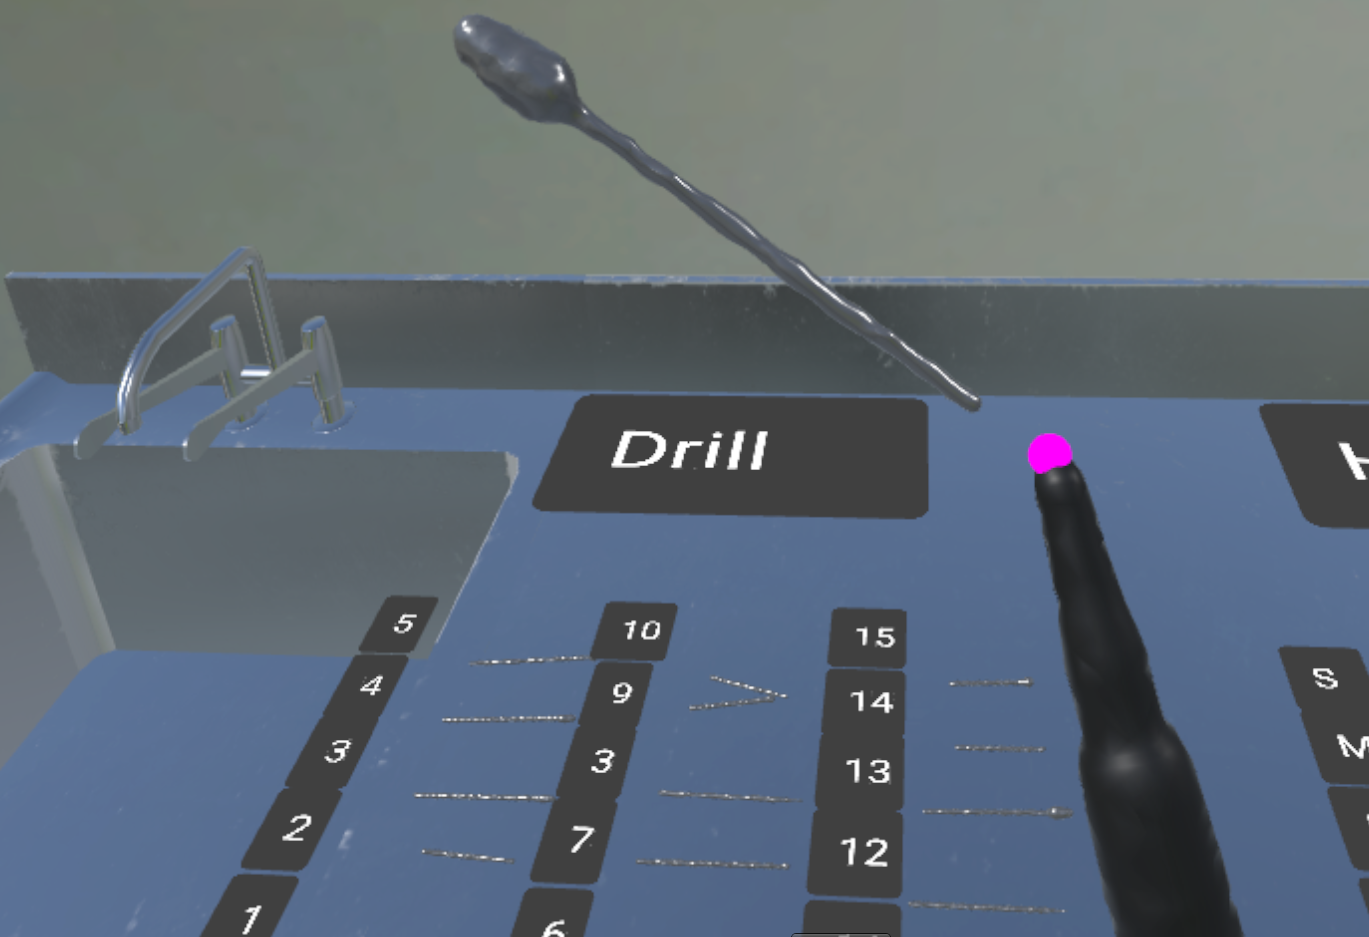
\includegraphics[width=200px]{images/implementation/features/procedures/drilling_attachment.png}
    \caption{\label{fig::FeatureDrillingAttachments}Process of attaching drill bit to the drill handle. With the right hand, the user performs the indicate action by touching 
    the respective button. With the other hand, the bit is picked up by grabbing it and moved into the pink sphere to attach the attachment.}
\end{figure}

In total, there are fifteen bits which can be used as an attachment for the drilling procedure.
Bits are modeled after their real counterparts in UHA.
They differ in size, length and width.
A visual signal is shown to the user while the indicate action is performed on the hand holding the drill handle.
By moving a drill bit to the visual indicator, the bit is attached to the handle (Figure \ref{fig::FeatureDrillingAttachments}).
Swapping out bits is performed by simply moving another bit into the indicator.
To perform the procedure, the drill handle must have a bit attached. 

\begin{figure}[ht]
    \centering
    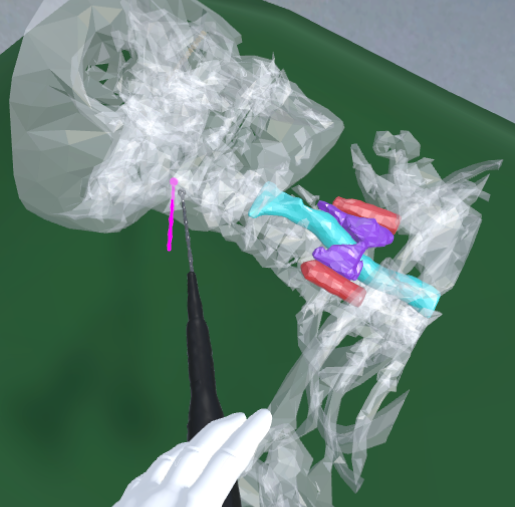
\includegraphics[width=200px]{images/implementation/features/procedures/drilling.png}
    \caption{\label{fig::FeatureDrilling}Drilling procedure. The pink object represents the last performed step, which was performed using the currently selected tool by pressing 
    the respective button all the way.}
\end{figure}

By triggering the perform action of the hand holding the drill, a copy of the currently attached drill bit is created and added to the project case. 
This copy has a different material, i.e. a pink material, to indicate that it is part of the project case (Figure \ref{fig::FeatureDrilling}).
Additionally, textual information about the currently attached drill bit will be stored in the project case, so that the exact procedure can be reproduced later (Requirements \ref{req::N3}, \ref{req::N5}).
The drill bit will not be removed on performing a procedure, so that multiple drilling steps can be performed consecutively.
When the drill is no longer needed, it can either be placed back on the instrument tray or the operating table for quick access.
Note that any instrument, excluding the osteosynthesis plates described later, can be placed anywhere in the OT.
\paragraph{Chiseling}

The \textbf{chiseling} procedure has two parts to it.
First, with one hand a chisel has to be chosen.
Users have a choice between a small, medium, large and extra large chisel to perform the procedure.
With the other hand, users then have to pick up the hammer.
Since this procedure requires users to hold two surgical instruments at the same time, this procedure can get cumbersome.
However, users can easily avoid this by placing the instruments on the operating table in the middle of the OT and repositioning afterwards (Figure \ref{fig::ChiselPrepare}).

\begin{figure}[ht]
    \centering
    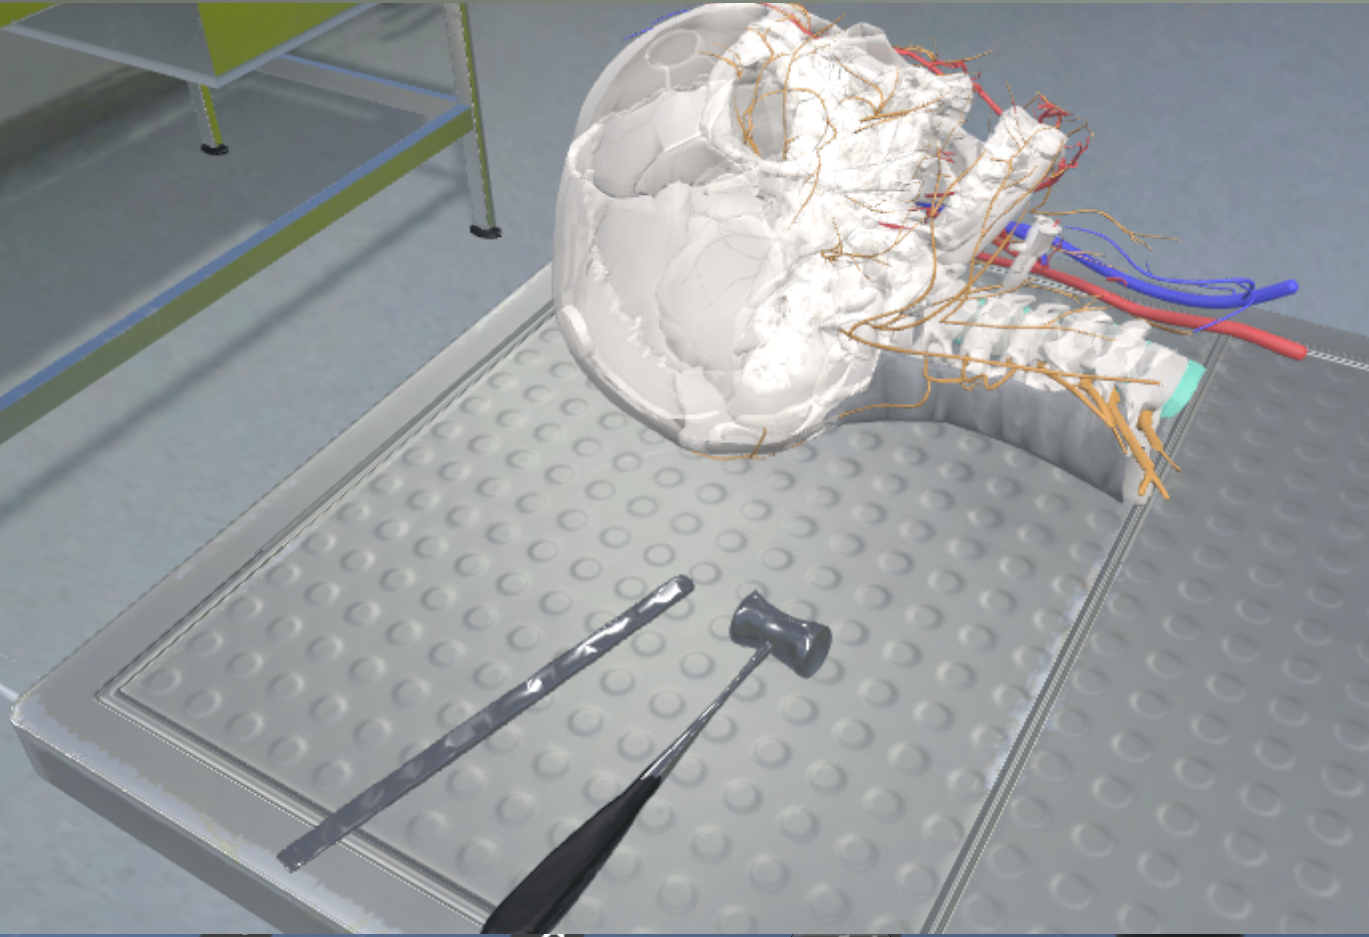
\includegraphics[width=\linewidth]{images/implementation/features/procedures/chisel_prepare.png}
    \caption{\label{fig::ChiselPrepare}The user prepares for the chiseling procedure by placing the instruments on the OT where the patient is located.
    indicators with the hammer in the other hand to perform the procedure.}
\end{figure}

When users have the perfect viewpoint, they can take up both instruments once again and start the procedure.
By pressing the indicate button on the hand where the chisel is located, rectangular indications at the top and bottom end of the chisel are shown to the user.
While these indications are active, the user has to perform a hammering motion with the hand holding the hammer.

\begin{figure}[ht]
    \centering
    \begin{minipage}{.5\textwidth}
      \centering
      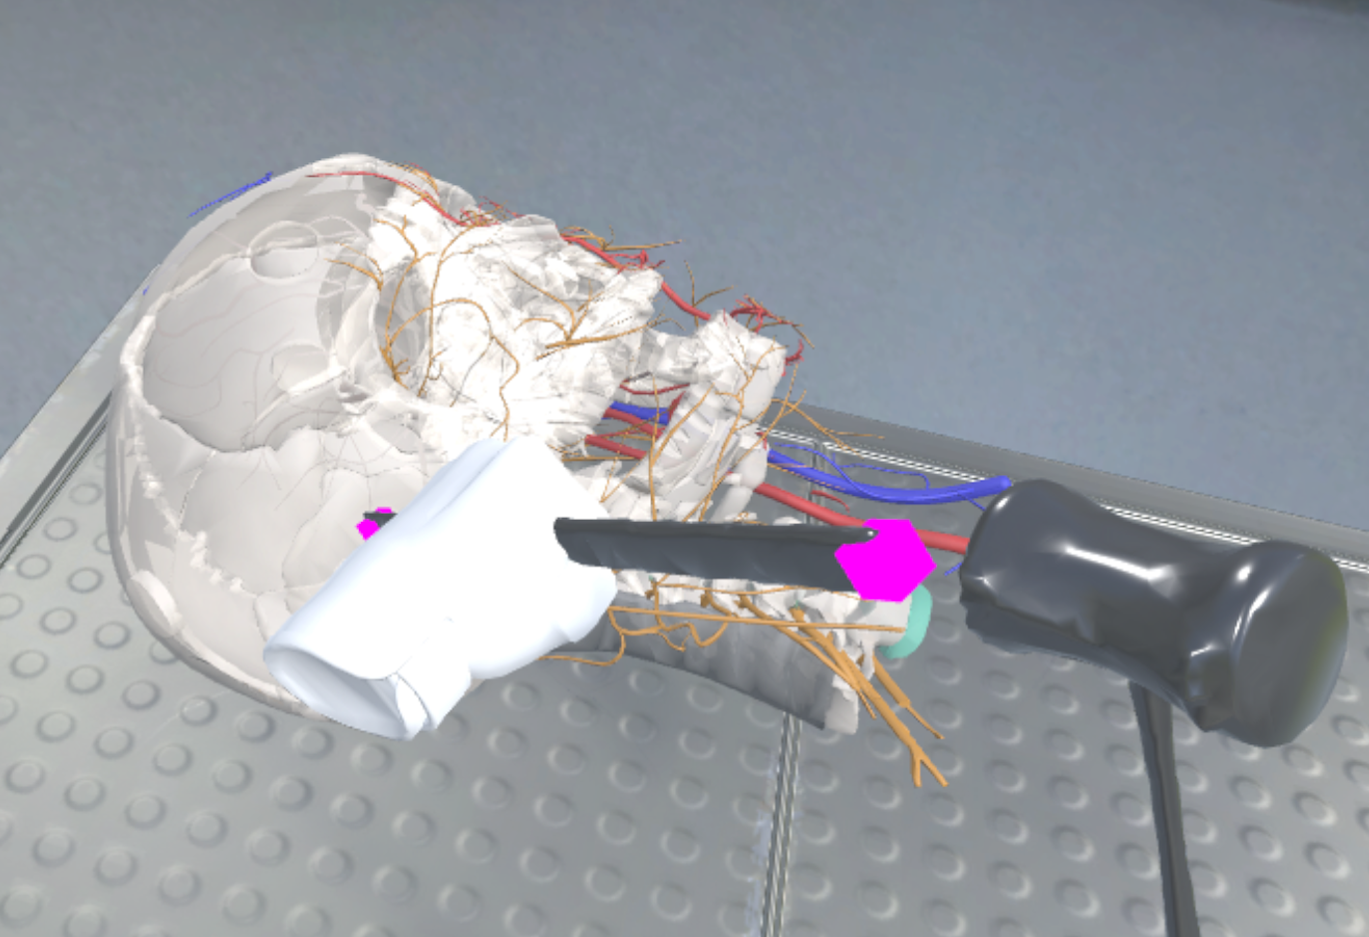
\includegraphics[width=0.99\linewidth]{images/implementation/features/procedures/chisel_1.png}
    \end{minipage}%
    \begin{minipage}{.5\textwidth}
      \centering
      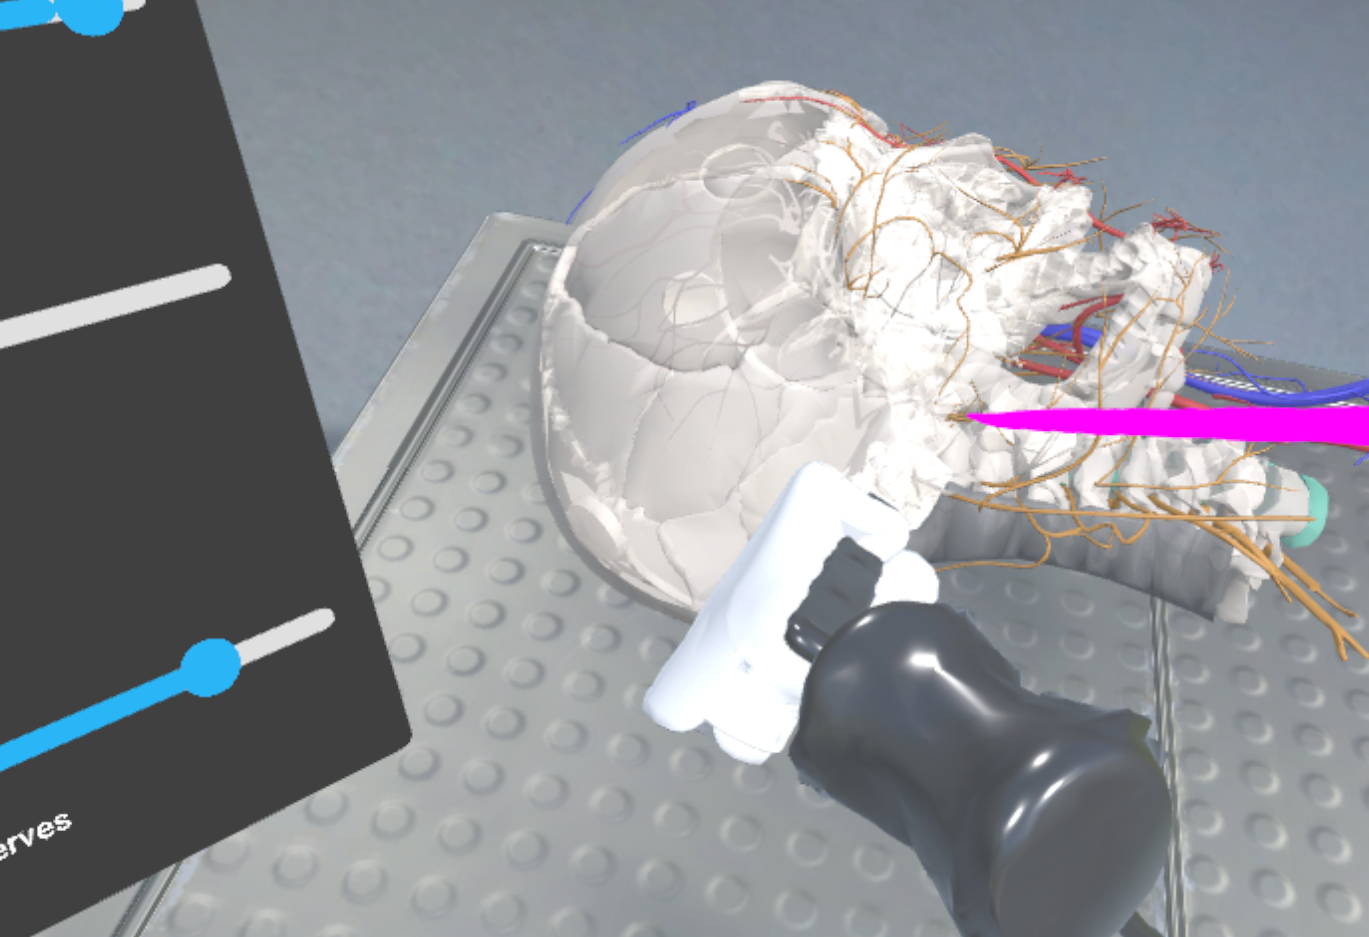
\includegraphics[width=0.99\linewidth]{images/implementation/features/procedures/chisel_2.png}
    \end{minipage}
    \caption{\label{fig::ChiselProcedure}Process of the chiseling procedure. Left: The users uses the indicate action with his left hand in preparation for the procedure. Right: After hammering on the indication on the chisel, the procedure has been performed and a step is generated.}
\end{figure}

When they hit the rectangular indicators located on the chisel, the chiseling procedure step is added to the project case in form of a modified copy of the hold chisel (Figure \ref{fig::ChiselProcedure}).
Here, information about the performed step is also included in the form of chisel size used for the procedure. 
\paragraph{Sawing}

\begin{figure}[ht]
    \centering
    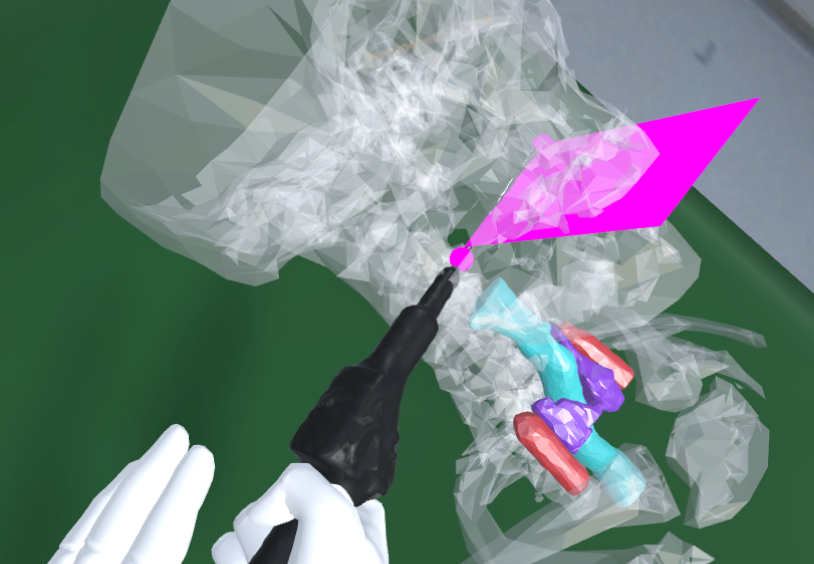
\includegraphics[width=200px]{images/implementation/features/procedures/bonesaw.png}
    \caption{\label{fig::FeatureBoneSaw}Bonesaw Procedure}
\end{figure}

The \textbf{sawing} procedure is performed by picking up the bonesaw.
Touch the controller will show two indications to the user (Figure \ref{fig::FeatureBoneSaw}).
The procedure is performed by first pressing down the trigger button and then letting go of it.
When letting go of the trigger button, a two dimensianal plane is created in the three dimensional space by using four points.
Two of these points are created when pressing down, and the other two when letting go of the trigger button.
A plane is then created with which the user can reproduce the way in which the bonesaw has been moved.
Arbitrary cutting shapes can be created by breaking them down into two-dimensional shapes and performing multiple movements.
\paragraph{Milling}

\begin{figure}[ht]
    \centering
    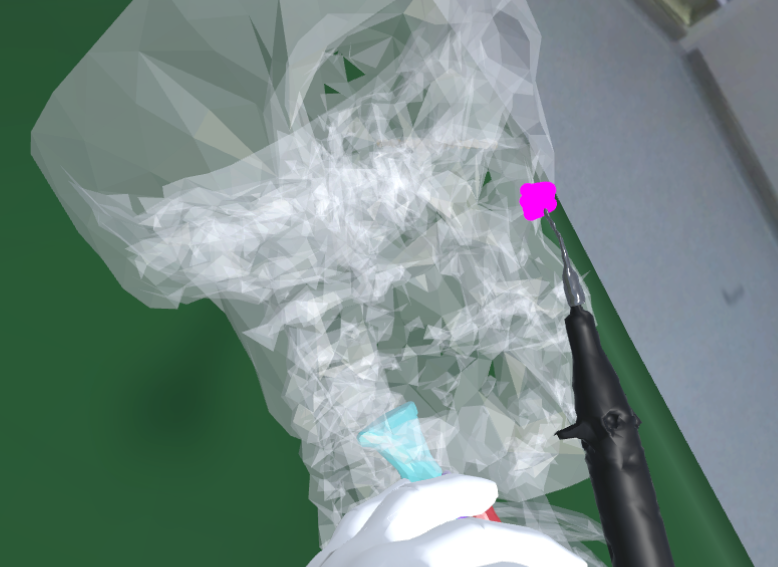
\includegraphics[width=200px]{images/implementation/features/procedures/piezo.png}
    \caption{\label{fig::FeaturePiezo}Milling procedure. Holding down the trigger button will draw little spheres until the button is released. The resulting object represents the volumetric space which is to be milled.}
\end{figure}

The \textbf{milling} operation is performed by grabbing the piezo instrument.
The indicator for the piezo is at the tip of the instrument, indicating which area will be milled.
While the "perform" button is being held down, little spheres are being drawn at the tip of the instrument \ref{fig::FeaturePiezo}.
When the button is released, the shapes are combined into a single 3D model and added as a project step.
The resulting object represents the volumetric space which has to be milled in the procedure.
The procedure can be reconstructed by "milling" the same 3D space in the virtual operating room.
\begin{figure}[ht!]
    \centering
    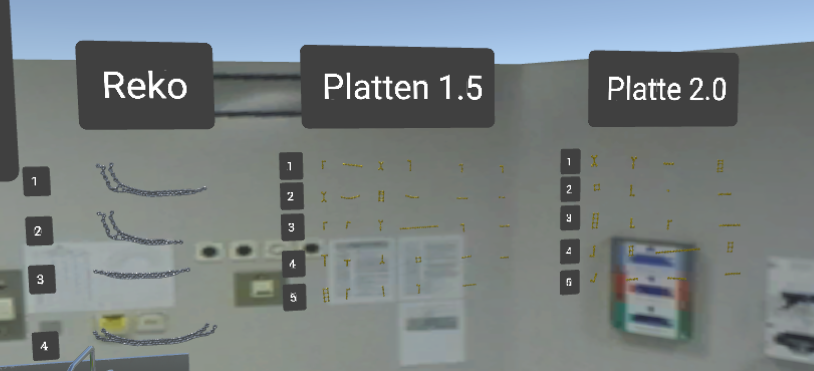
\includegraphics[width=\linewidth]{images/implementation/features/procedures/metal_plates_1.png}
    \caption{\label{fig::FeatureMetalPlate} Osteosynthesis Plates Overview}
\end{figure}

The osteosynthesis plates procedure consists of two steps before adding it as a step to the project case.
First, users have to chose which plate to use (Figure \ref{fig::FeatureMetalPlate}).
The user can chose from four reconstruction plates, 29 1.5mm plates and 20 2.0mm plates (Firma Angeben, osteosynthesis plates).
The optimal plates to use vary due to the pathology of the patient and the previously performed procedures.
After selecting the proper plate, a number of indicators will show to the user (Figure \ref{fig::FeatureMetalPlate2}).
In the context of the osteosynthesis plates, these indicators are "control points", with which the user can bend and twist the plates.
Bending and twisting is performed by chosing a control point via hovering them with the users free hand and grabbing them.
Then, the user has to translate and rotate the control point in the desired manner.
\begin{figure}
  \centering
  \begin{minipage}{.5\textwidth}
    \centering
    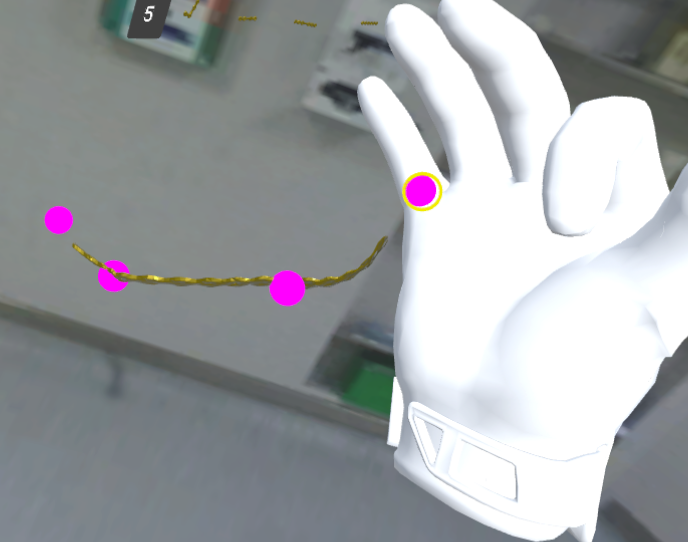
\includegraphics[width=0.95\linewidth]{images/implementation/features/procedures/metal_plates_2.png}
  \end{minipage}%
  \begin{minipage}{.5\textwidth}
    \centering
    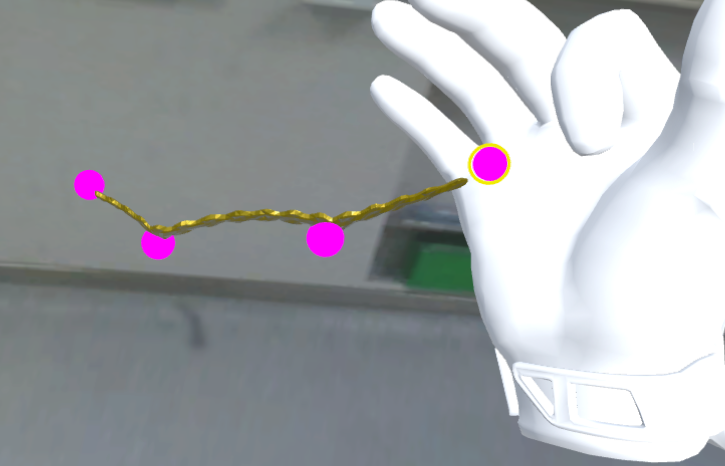
\includegraphics[width=0.95\linewidth]{images/implementation/features/procedures/metal_plates_3.png}
  \end{minipage}
  \caption{\label{fig::FeatureMetalPlate2}Osteosynthesis Plates Modifications. User can translate and rotate "control points" to perform modifications to the plates shape} 
\end{figure}

The user can then observe in which way this has affected the shape of the metal plate and either position the plate on the patient or perform more modifications to the plates via controlpoints.
The correct modification of the metal plates differs quite a lot from real life modifications to the plates.
However even though there is a slight learning curve to it, the modification is consistent and predictable (Figure \ref{fig::FeatureMetalPlate2}).


\begin{figure}[ht!]
    \centering
    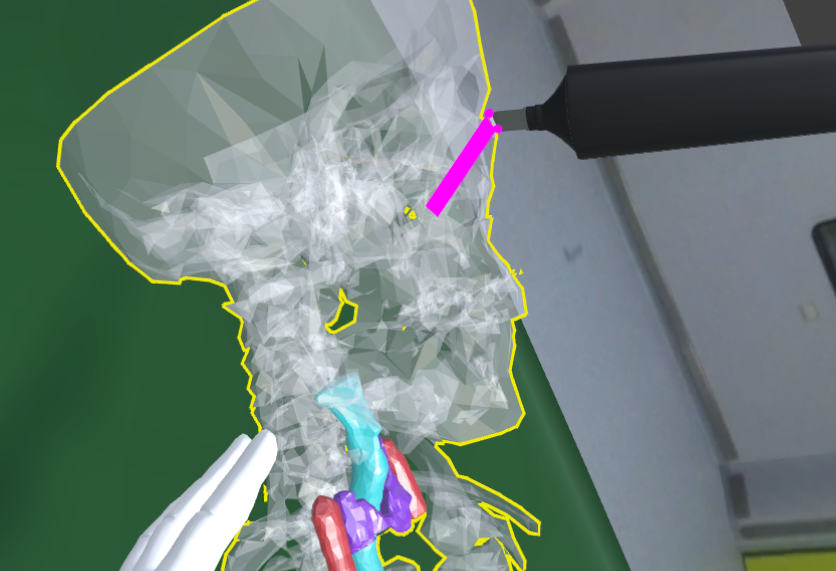
\includegraphics[width=\linewidth]{images/implementation/features/procedures/marker.png}
    \caption{\label{fig::FeatureMarker}Marker Procedure}
\end{figure}

The marking procedure is similar to the bonesaw procedure, meaning that rectangular shapes are drawed into the three dimensianal space (Figure \ref{fig::FeatureMarker}).
However, here the created shapes are much thinner.
In contrast to the bonesaw, the virtual hands of the user are also disabled here.
This way, the user can decide to hold the marker in the optimal way.
Since the main objective is marking specific spots on the patient, this is the natural approach.

\subsection{\label{sec::RelatedWorkDiscussion}Discussion - Pros and Cons}
In 2009, Swennen et al. discuss several improvements for three-dimensional treatment planning over conventional methods \cite{swennen2009three}.
Cost reduction and better patient outcome were achieved with three-dimenstional treatment planning, even though the planning was still conducted on conventional computers with 2D screens.
Additionally, experts all over the world can be consulted since treatment plans can be send via electronic mail.
Especially the diagnosis, treatment planning and treatment communication were improved \cite{swennen2009three}.

Virtual reality would offer advantages such as 3D stereoscopic vision, scalability, and repeatability over traditional methods such as described in \ref{chap::Introduction}.
As mentioned by Hassfeld et al \cite{HASSFELD20012}, developed software has a strong need to be easily accesible.

Kim et al (2017) presented that immersive VR combined with 3D printing models improved visualization and interaction with complex anatomy, surgical rehearsal, customization, and precise communication between medical specialists \cite{.2017}.
Furthermore, the authors argue that VR systems will improve model manipulation and provide more anatomical information for each stage of the surgical procedure over traditional techniques \cite{.2017}.

Pulijala et al (2017) concluded that when the context of simulation closely resembles a real-life model, such as an operating room environment, learning was found to be better \cite{Pulijala.2017}.
The authors stress that Oculus Rift and HTC Vive-like devices brought high-quality surgical simulations into common man’s reach \cite{Pulijala.2017}.
\newline
Pulijala et al describe how technical and non-technical skills have to be acquired in surgical training.
Traditional means of surgical education though hands-on-practice has been around for more than a century.
It was found that four out of ten novice surgeons are not confident in performing major procedures.
VR Surgery aims to provide cognitive training for oral and maxillofacial surgeons \cite{RN68}.

Parham et al (2019) presented how VR can be used as a low-cost training tool.
By developing a low cost simulation, using commercially available VR software and the Oculus Rift HMD, they have succesfully helped surgeons to prepare for radical abdominal hysterectomy surgery procedures in Zambia \cite{Parham.2019}.
The authors presented a simulator which succesfully created pre-trained novices by providing new ways to acquire the psycho-motor skills, sensory acuity and cognitive planning abilities needed for sugery.
Virtual reality based training has proven to reduce the time to acquire surgical proficiency \cite{RN61,RN62}. 
In randomized control studies, VR trained trainees performing laparoscopic cholecystectomy, made fewer errors and were faster \cite{RN63,RN64}.
VR trained trainees required only half the time to reach the skill level of intermediately skilled surgeons compared to standard training.
Hence, it is proven that skills acquired in simulations can successfully be translated to the operting theatre (OT) \cite{RN63,RN64}.
Parham et al recognize a need for clinical testing to establish VR efficacy, since there is a lack of research for VRs clinical utility \cite{RN59}. 

Swennen et al (2009) mention how one of the biggest disadvantage of this technology, having a powerful enough workstation to power the software, will soon be eliminated \cite{swennen2009three}.
Today, the trend is already  affortable, consumer friendly HMDs.
Standalone HMD such as the Oculus Quest also propose an interesting application area for surgery, where cost of high-end computer hardware is eliminated. 
However, as of now, this technology is not powerful enough for surgical simulation.

Sampogna et al (2017) confirm the feasability of preoperative and intraoperative guidance by virtual 3D models \cite{Sampogna.2017}.
For patient specific models however, good-quality radiologic imaging is a concern.
Additionally, the process of segmentation can be time consumer, although it depends on the proficiency with available tools such as 3D Slicer.
The authors demonstrated the feasability and clinicians appreciation for VR in surgery \cite{Sampogna.2017}.

Commercial VR will advance significantly in the future, allowing for an even better adoption of VR simulations in surgery.
Surgical training enhanced with augmented and virtual reality will have wide applications according to Parham et al \cite{RN61,RN62}.
However, such technology has to be carefully build and clinically tested.
VR and AR has the potential to help train the workforce and to ensure higher quality standards \cite{RN52}.

Barber et al (2020) mention the steep learning curve of developing VR applications as a disadvantage.
The point out that even though VR is an established technology as of now, there is still no definition on how to effectively use tools and features to create educational applications \cite{Barber.2020}.
Even though the aforementioned drawback, the authors conclude that VR simulation using game engines is feasible and will be established in future studies.
This thesis confirms the feasibility of using game engines, in this case Unity3D, for bringing educational value through creating surgical simulations.